
\documentclass{article}

\usepackage{tikz,pgfplots}
\pagestyle{empty}

\title{Machine Learning: Project 1} 
\author{Cody Worsnop}
\date{\today}

\begin{document}

\maketitle 

\section*{Overview} % Unnumbered section

As a documentation overview, I'll provide key functions and their general implementation. I'll do my best to discuss design and implementation strategies for the overall problem as well. 
\newline
\newline
\bf Note: \rm
My network is a rather slow learner. Be patient, it'll come around, it's just a bit shy. 

\section*{Calculate Loss} % Unnumbered section

The loss for this project is given by the formula 

\begin{equation}
L(y, \hat{y}) = -\frac{1}{N}\sum_{n\in{N}}\sum_{i\in{C}}y_{n,c}\,Log\,\hat{y}_{n,i}
\end{equation}

So for every prediction, we are summing each class and each value in each class. For example, if we have a softmax prediction of <0.4, 0.6> then the loss function would be (0 * 0.4) + (1 * 0.6). As a side affect, we are only concerned with the correct prediction. This is a property of cross-entropy loss. 

My implementation runs the prediction function and then runs the above formula on all the predictions. Once done, the final error is returned. 

\section*{Predict} 

For this project, I have numerous prediction functions. This is due to the orignal write up for the project only specifying that one feature be passed in at a time in the function. Thus, I have the following functions: 

\textbf{predict(model, x)}

This is the normal prediction function as designed in the project report. It runs foward propagation on a single feature and returns the prediction of the network. 

\textbf{predict\_many(model, X, outputSize=2)} 

This is the predict many function that takes the entire feature vector and returns the prediction for all the features in one large vector. 

\section*{Build Model} 

Build model is where all the business happens. For every epoch (num\_passes) we predict all of the features, output the loss if necessary, and run gradient descent on the network. All the weights and biases, including the different activations (a, h, and z) are saved in a dictionary that get's populated at the start of build model. 

\section*{Build Model 691}

This function extends the functionality to three outputs. This was a rather straightforward process once build\_model was done. Mostly, changes were making the matrix dimensions for the weights and biases to 3 instead of 2. Also, I reused my predict\_many function from above by using the outputSize parameter. 

\section*{plots} 

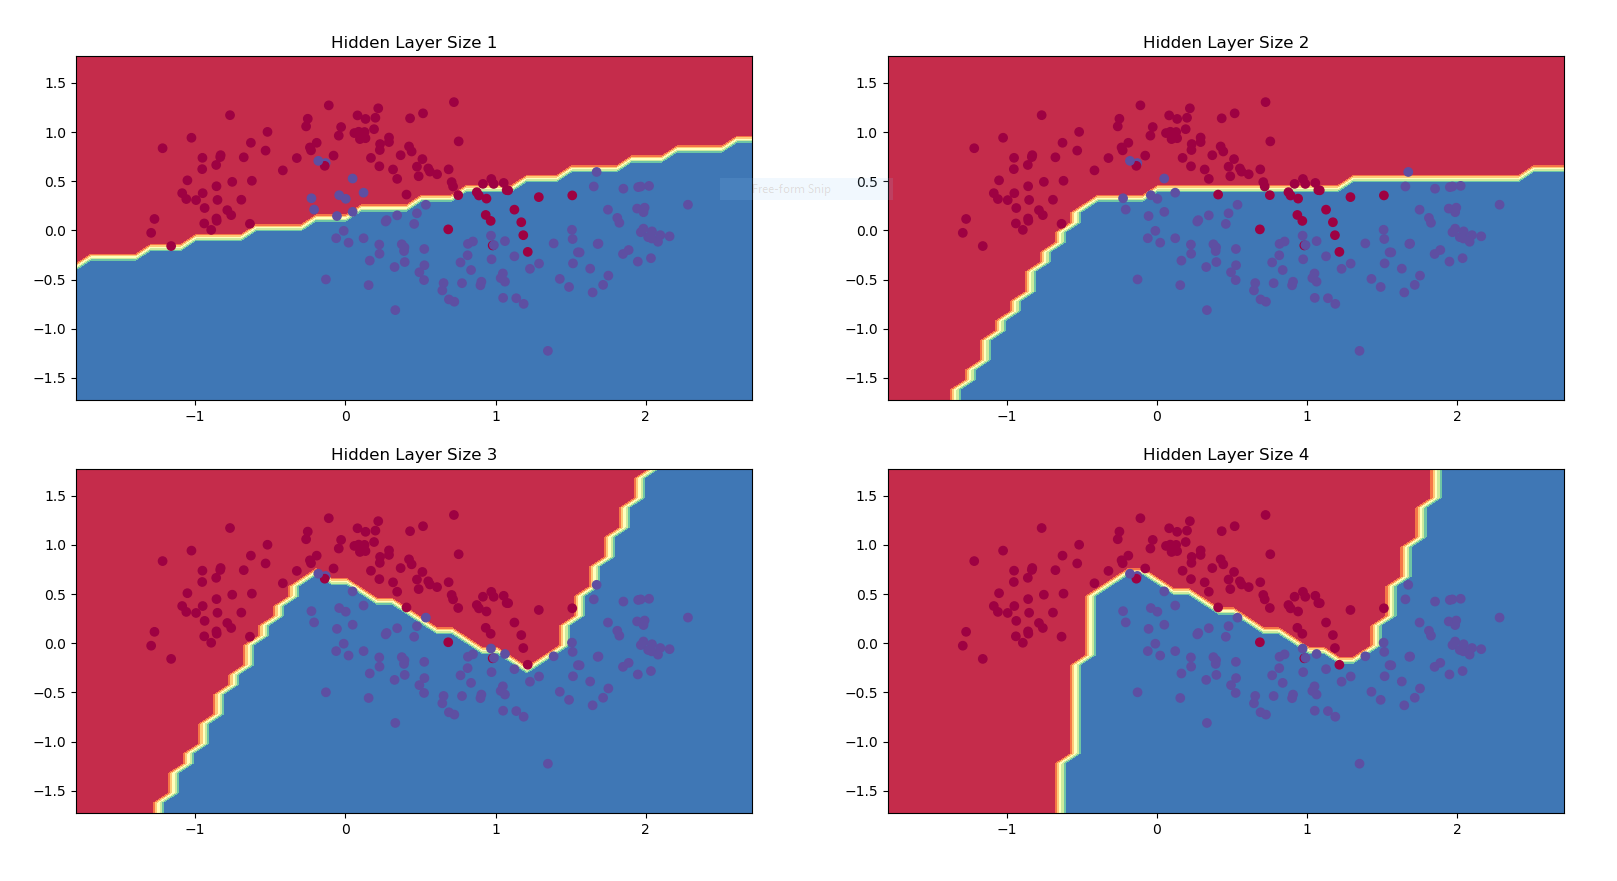
\includegraphics[width=\textwidth]{nn.png}

\end{document}
